\documentclass[12pt]{exam}
%\documentclass[12pt]{article}
\usepackage[letterpaper, margin=0.75in]{geometry}
\usepackage{graphicx}
\usepackage{enumitem}
\usepackage{booktabs}
\usepackage{amsmath}
\usepackage{tabularx}

\begin{document}
\footer{}{Page \thepage\ of \numpages}{}


\begin{flushright}
\makebox[0.5\textwidth]{\large Name:\enspace\hrulefill}
\vspace{0.2in}

\makebox[0.5\textwidth]{\large Date:\enspace\hrulefill}
\end{flushright}

\begin{center}

\includegraphics[width=10cm]{../images/logo.png}
\end{center}


\begin{center}
\noindent{\LARGE Conceptual Physics \\ Class 3 Questions \\ Feb 16, 2018\\}
\end{center}
\vspace{0.2in}

\clearpage

\begin{questions}
\question
A passenger on a cruise ship finds, while the ship is docked, that he can leap off the upper deck and just barely make it to the pool on the lower deck. If the ship leaves dock and is cruising rapidly, will this adrenaline junkie still be able to make it?

From: \textit{Light and Matter}, Ch.2, Discussion Question B
\vspace{1in}

\question
Suppose that a juggler is in a bus traveling on the highway at 65 mph. The juggler throws a ball \textbf{vertically} up in the air. 


\begin{parts}
\part Which of the following pictures best represents the trajectory of the ball, \textbf{as seen by the juggler}?

\begin{center}
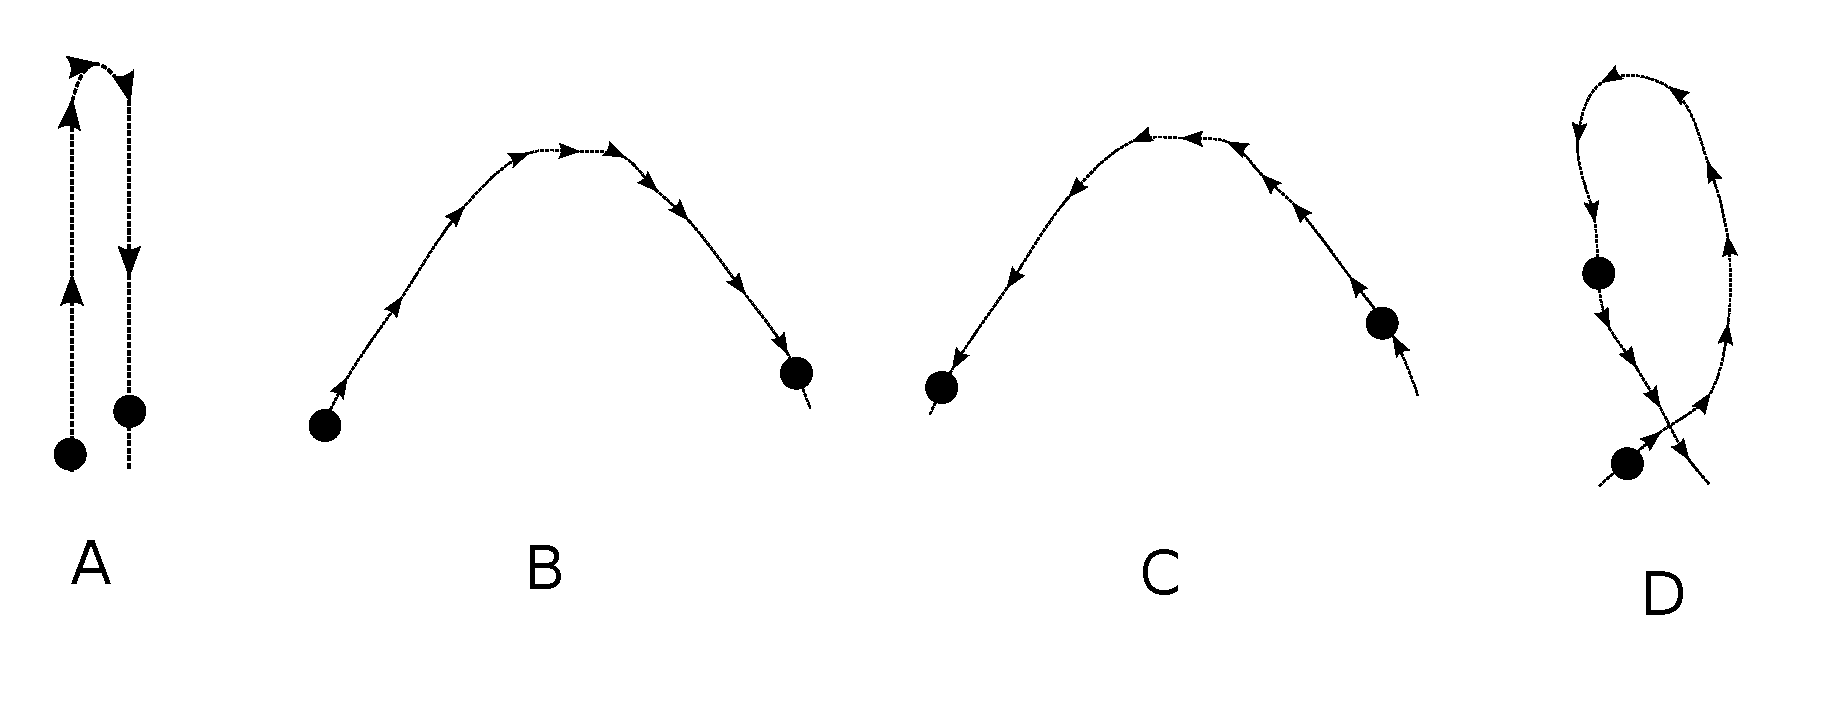
\includegraphics[width = 0.5\textwidth]{../images/Ball_Juggler.pdf}
\end{center}

\part Now, suppose someone is standing on the side of the highway and watches the bus go by, moving from her left to her right, just as the juggler throws the ball. Which of the following pictures best represents the trajectory of the ball, \textbf{as seen through the bus's windows by this bystander}?

\begin{center}
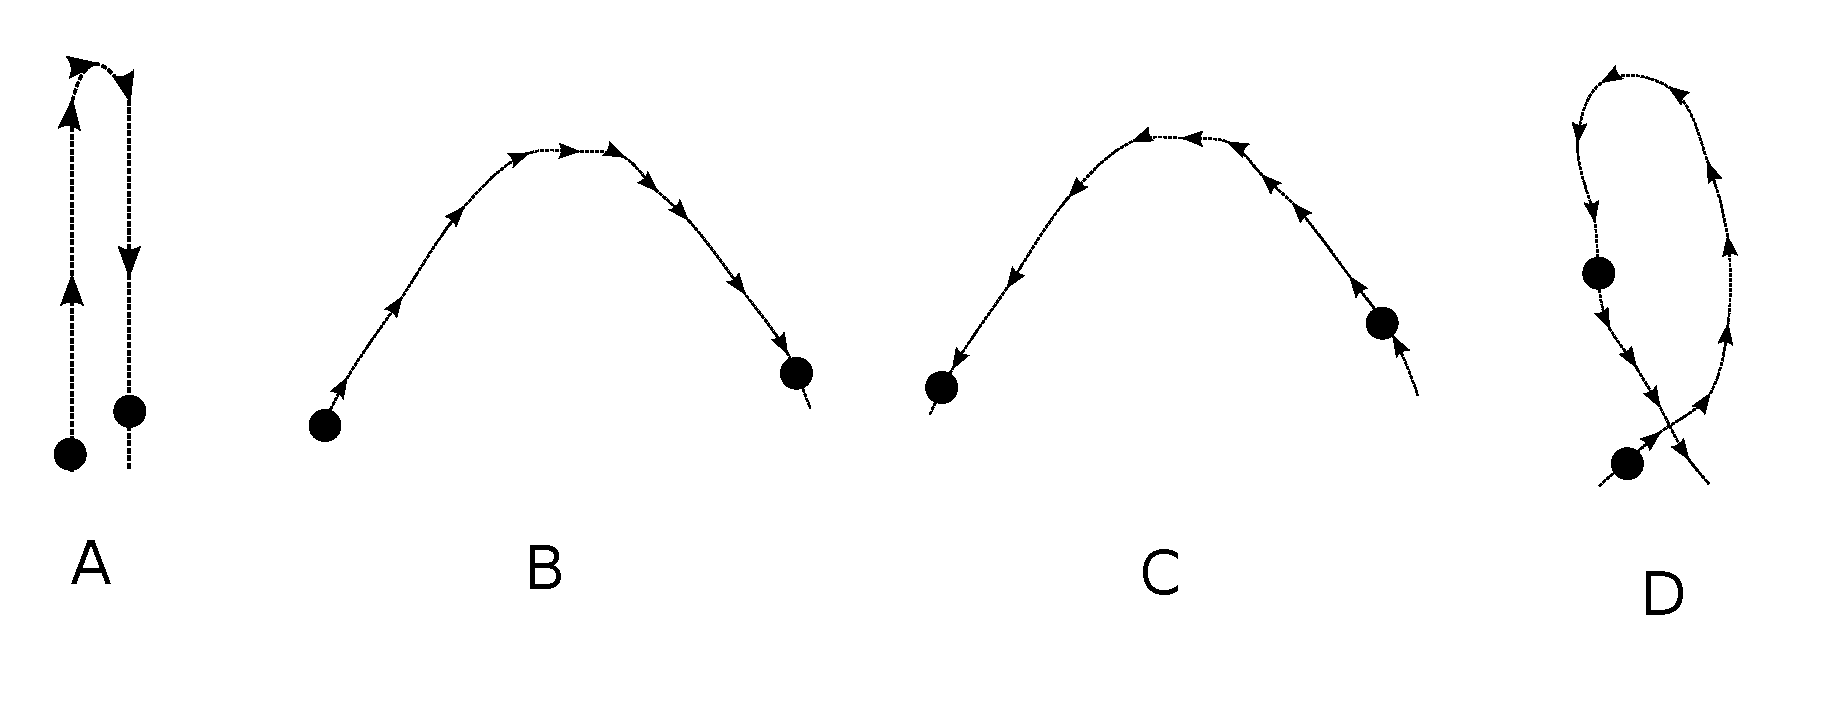
\includegraphics[width = 0.5\textwidth]{../images/Ball_Juggler.pdf}
\end{center}

\end{parts}


\question
Consider the following argument that was made by someone trying to show that the Earth is not a spinning globe but rather a flat, stationary surface:

Suppose that I set up a target 1200 ft away from me, due East, and shoot at it with a rifle using bullets that travel at 1200 feet-per-seconds. Then I will, of course, hit the target one second after firing. But science tells us that the Earth is spinning at 1500 feet-per-seconds from West to East. So if I shoot East, my bullet will travel 1200 feet in one second, but the target which is on the Earth will move away 1500 feet in that one second. Therefore, I could never hit my target because the Earth moves faster than the bullet in that direction. This is what should happen on a spinning globe that some of you claim to live on.

What do you think?

\clearpage

\question
In the following scenarios, draw an arrow indicating the direction of \textbf{velocity} and another indicating \textbf{acceleration}.

\begin{parts}

\part A car on the highway.

\begin{table}[h!]
     \begin{center}
     \begin{tabularx}{\textwidth}{ |X | X | X | }
      A car is cruising at a constant speed of 70~miles/hour on the highway. & In order to pass a slow moving truck, the driver applies the gas to increase her speed to 80~miles/hour. & Noticing traffic up ahead, the driver applies the break to slow down. \\ 
     ~ & ~ & \\
     
     \raisebox{-\totalheight}{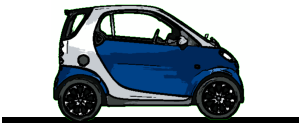
\includegraphics[width=0.3\textwidth]{../images/caronRoad.pdf}}
      & 
      \raisebox{-\totalheight}{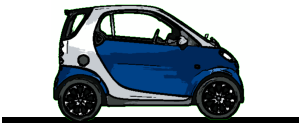
\includegraphics[width=0.3\textwidth]{../images/caronRoad.pdf}}
      & 
      \raisebox{-\totalheight}{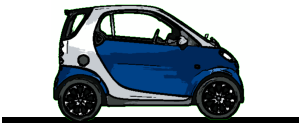
\includegraphics[width=0.3\textwidth]{../images/caronRoad.pdf}}
      \\
      \end{tabularx}
      \end{center}
\end{table}
\vspace{0.3in}

\part A ball being tossed up off a cliff.
\begin{table}[h!]
     \begin{center}
     \begin{tabularx}{\textwidth}{ |X | X | X | }
      As the person is tossing it up (while they are still in contact). & When the ball reaches the highest point in its trajectory. & As the ball is falling down the edge of the cliff. \\ 
     ~ & ~ & \\
     
     \raisebox{-\totalheight}{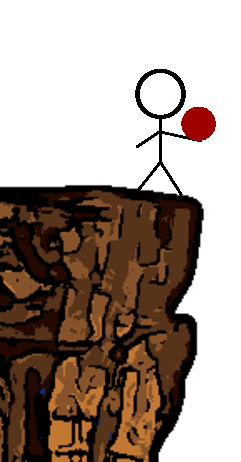
\includegraphics[width=0.2\textwidth]{../images/balltossUp.pdf}}
      & 
      \raisebox{-\totalheight}{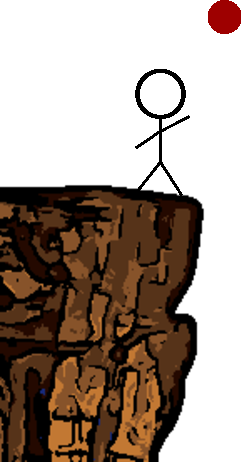
\includegraphics[width=0.2\textwidth]{../images/balltossTop.pdf}}
      & 
      \raisebox{-\totalheight}{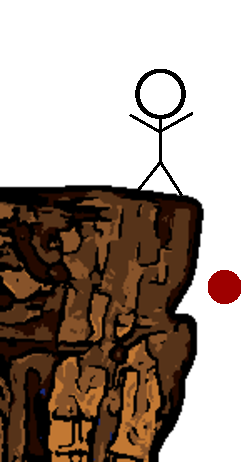
\includegraphics[width=0.2\textwidth]{../images/balltossDown.pdf}}
      \\
      \end{tabularx}
      \end{center}
\end{table}
\end{parts}

\clearpage
\question
There are different units with which to measure distance. For instance, a light-year is the distance travelled by light in a vacuum during the course of one year. The Earth is 8 light-minutes away from the Sun, meaning light takes 8 minutes to reach the Earth from the Sun (so in effect, what we are seeing is the Sun time-delayed by 8 minutes).

\begin{parts}
	\part If the speed of light is $3.0 \times 10^8$~m/s, then what is the Earth's distance in meters to the Sun?
	\vspace{0.7in}
	\part What distance does the Earth travel in one year? (Assuming it follows a perfect circle).
	\vspace{0.7in}
	\part What is the Earth's speed as it revolves around the Sun? 
	\vspace{0.7in}
	\part What is the Earth's displacement during one year?
	\vspace{0.7in}
	\part What is the Earth's average velocity during one year?
\end{parts}
\vspace{0.8in}
\begin{center}
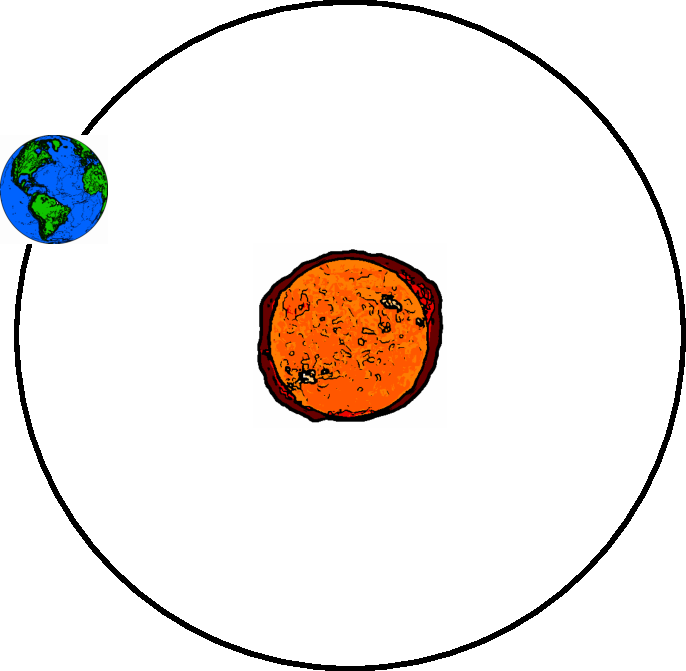
\includegraphics[width = 0.4\textwidth]{../images/earthSun.pdf}
\end{center}


\clearpage

\question
You are driving along a highway and pass a mile marker, which reads 81.0. Five minutes later, you pass mile marker 76.0. Assume you neither braked nor accelerated (say, because you are using cruise control).
\begin{parts}
	\part What is your speed in miles/hour?
	\vspace{0.5in}
	\part What is your speed in km/hour?(1 mile = 1.6 km)
	\vspace{0.5in}
\end{parts}

\question
A measure of a car's performance is how fast it can reach 60 miles/hour from rest. The new Tesla Model S P100DL can accelerate from rest to 60 miles/hour in 2.27 seconds. Assuming it travels in a straight line,

\begin{parts}
	\part What is its acceleration (assuming it is constant during this time)?
	\vspace{0.5in}
	\part How far does it travel during this time?
	\vspace{0.5in}
	\part What is its average velocity?
	\vspace{0.5in}
\end{parts}

\question It's a sunny Sunday afternoon, about 65$^{\circ}$F, and you are walking around the reservoir in Central Park enjoying the last of the autumn color. The sidewalk is crowded with runners and walkers. You notice a runner approaching you wearing a tee-shirt with writing on it. You read the first two lines, but are unable to read the third and final line before he passes. You wonder, ``Hmm, if he continues around the reservoir, I bet I'll see him again, but I should anticipate the time when we'll pass again.'' You look at your watch and it is 3:07 p.m. You recall the reservoir is 1.58 miles in circumference. You estimate your walking speed at 3 miles per hour and the runner's speed to be about 7 miles per hour.
\begin{parts}
\part Draw a sketch of the problem.
\vspace{3in}
\part List the quantities that are relevant to solve this problem.
\vspace{1in}
\part Solve the problem, showing your work.
\vspace{2in}
\end{parts}

\end{questions}

\end{document}

